\chapter{Chimie du solide~: bandes, défauts et semi-conducteurs}\label{ch:b3:solid-state}

Un panneau solaire sur un toit et la diode électroluminescente d'une lampe
sont faits du même genre de cristal, du silicium ou un composé du gallium
avec l'azote, l'arsenic ou le phosphore, dans lequel on a introduit
volontairement quelques atomes d'impureté par million. Leur fonctionnement
repose sur deux choses qu'une molécule ne possède pas~: des bandes de
niveaux d'énergie, séparées par un intervalle dont la largeur fixe la
lumière qu'un cristal absorbe ou émet, et des défauts, qui portent les
charges. Ce chapitre construit les bandes à partir des orbitales
moléculaires, dénombre les porteurs d'un \omterm{def:b3:solid-state:classes}{semi-conducteur}, et traite les
atomes manquants ou déplacés comme des espèces chimiques dotées de leurs
propres équilibres, jusqu'à l'\omterm{def:b3:solid-state:ionic-conductor}{électrolyte solide} de la sonde à oxygène d'un
pot d'échappement.

\begin{recall}
Le volume de première année a défini les cristaux, la liaison métallique,
les cristaux ioniques et covalents, les sites interstitiels et les alliages,
ainsi que l'équation de Nernst~; le volume de deuxième année, la méthode de
Hückel et l'intégrale de résonance $\beta$. Le
\cref{ch:b3:x-ray-diffraction} a donné le \omterm{def:b3:x-ray-diffraction:reciprocal}{réseau réciproque} et le
\cref{ch:b3:partition-functions} la \omterm{def:b3:partition-functions:boltzmann}{distribution de Boltzmann} et l'\omterm{def:b3:partition-functions:statistical-entropy}{entropie
statistique} $S = k\ln W$.
\end{recall}

\begin{omfigure}
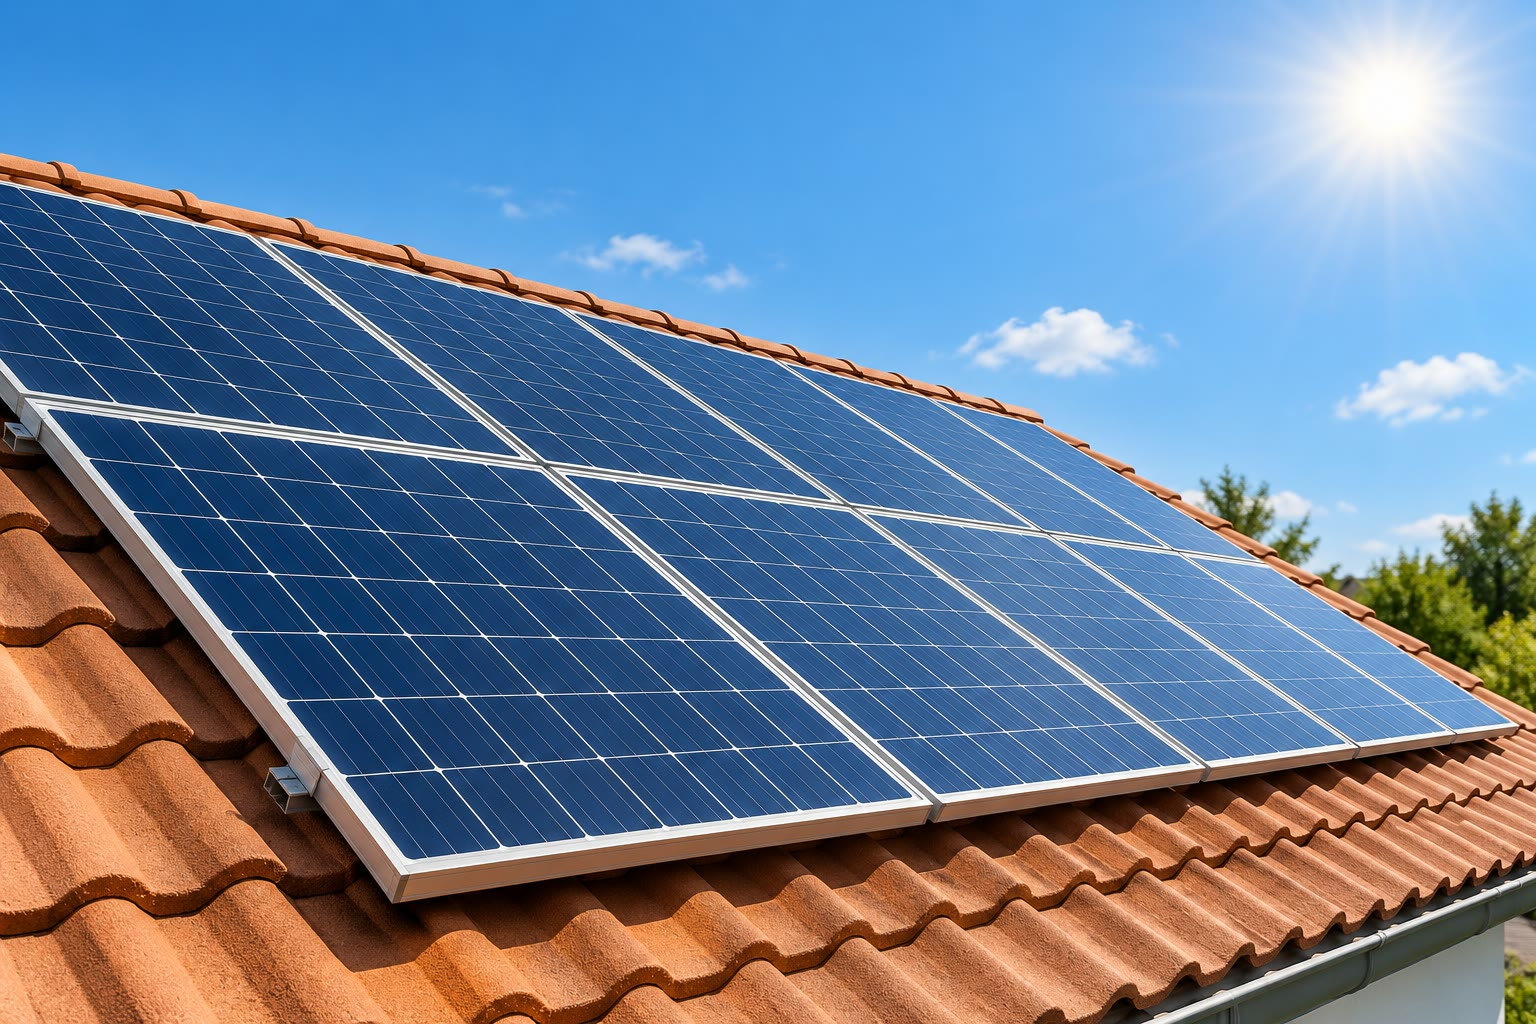
\includegraphics[width=0.6\linewidth]{images/book4/ai/b3-22-solar-panels.jpg}

{\small Panneaux solaires sur un toit de tuiles~: chaque cellule est une
fine tranche de silicium dans laquelle la lumière fait franchir aux
électrons une \omterm{def:b3:solid-state:band}{bande interdite} d'environ un électronvolt.}
\end{omfigure}

\section{Des orbitales aux bandes}

Prenons une chaîne de $N$ atomes identiques, portant chacun une orbitale s,
dans l'approximation de Hückel~: intégrale coulombienne $\alpha$ sur chaque atome, intégrale de résonance $\beta < 0$
entre voisins, nulle sinon.

\begin{theorem}[Niveaux d'une chaîne de Hückel]\label{thm:b3:solid-state:chain}
Les $N$ orbitales moléculaires d'une chaîne linéaire de $N$ atomes ont pour
énergies
\[
  E_k = \alpha + 2\beta\cos\frac{k\pi}{N + 1}, \qquad k = 1, \dots, N,
\]
avec des coefficients $c_j^{(k)} \propto \sin\bigl(jk\pi/(N + 1)\bigr)$ sur l'atome $j$. Quand $N \to \infty$, les niveaux
remplissent de façon dense l'intervalle de $\alpha + 2\beta$ à $\alpha - 2\beta$~: une bande de largeur $4|\beta|$.
\end{theorem}

\begin{proof}
Les équations séculaires s'écrivent $\beta c_{j-1} + (\alpha - E)c_j + \beta c_{j+1} = 0$ pour $j = 1, \dots, N$, avec $c_0 = c_{N+1} = 0$
(pas d'atome à ces places). Essayons $c_j = \sin(j\theta)$~: puisque $\sin((j - 1)\theta) + \sin((j + 1)\theta) = 2\cos\theta\sin(j\theta)$, chaque
équation devient $(\alpha - E + 2\beta\cos\theta)\sin(j\theta) = 0$, donc $E = \alpha + 2\beta\cos\theta$. La condition $c_0 = 0$ est vérifiée
pour tout $\theta$, et $c_{N+1} = \sin((N + 1)\theta) = 0$ impose $\theta = k\pi/(N + 1)$~; $k = 1, \dots, N$ donne $N$ niveaux
distincts (les autres valeurs les répètent ou s'annulent). Le plus bas et le
plus haut valent
$\alpha \pm 2\beta\cos(\pi/(N + 1))$, qui tendent vers $\alpha \pm 2\beta$~; l'écart entre voisins vaut au plus
$2|\beta|\pi/(N + 1)$, qui tend vers zéro.
\end{proof}

Pour $N = 2$, le théorème donne $\alpha \pm \beta$, les orbitales du système $\pi$ de l'éthène~; pour
$N = 6$, l'hexatriène à chaîne ouverte. En trois dimensions, il en va de même
pour toute sorte d'orbitale atomique~: les orbitales s donnent une bande s,
les orbitales p une bande p, et chaque bande contient $2N$ électrons pour
$N$ atomes.

\begin{definition}[Bandes]\label{def:b3:solid-state:band}
Une \emph{bande d'énergie}\index{bande d'energie@bande d'énergie} d'un cristal est un domaine
continu d'énergies monoélectroniques permises, formé à partir des orbitales
de tous ses atomes. Une \emph{bande interdite}\index{bande interdite} $E_g$ est un domaine d'énergies
dépourvu de niveaux entre deux bandes. Dans un \omterm{def:b3:solid-state:classes}{semi-conducteur} ou un \omterm{def:b3:solid-state:classes}{isolant}
à température nulle, la bande remplie la plus haute est la \emph{bande de valence}\index{bande de valence}
et la bande vide la plus basse la \emph{bande de conduction}\index{bande de conduction}.
\end{definition}

\begin{definition}[Densité d'états et niveau de Fermi]\label{def:b3:solid-state:fermi}
La \emph{densité d'états}\index{densite d'etats@densité d'états} $g(E)$ est le nombre de
niveaux par unité d'énergie (et par atome ou par unité de volume) au
voisinage de l'énergie $E$. Le \emph{niveau de Fermi}\index{niveau de Fermi} $E_F$ est l'énergie à laquelle un
niveau a une probabilité $1/2$ d'être occupé~; à température nulle, tous les niveaux situés au-dessous
sont remplis et tous ceux situés au-dessus sont vides.
\end{definition}

\begin{omfigure}
\begin{tikzpicture}
\begin{axis}[width=0.78\linewidth, height=6.2cm, xmin=0.3, xmax=7.6, ymin=-2.3, ymax=2.3,
  axis lines=left, xtick={1,2,3,4,5,6.6}, xticklabels={2,4,8,16,64,$\infty$~: $g(E)$},
  xlabel={nombre d'atomes $N$}, ylabel={$(E - \alpha)/|\beta|$},
  ytick={-2,-1,0,1,2}, tick label style={font=\small}, label style={font=\small}]
\addplot[only marks, mark=-, mark size=7pt, omDef, thick] table[x=col, y=e] {figdata/out/bachelor-3-band-chain.dat};
\addplot[omThm, thick] table[x expr=6.0+0.55*\thisrow{g}, y=e] {figdata/out/bachelor-3-band-chain-b.dat};
\draw[black!40, dashed] (axis cs:0.3,-2) -- (axis cs:7.6,-2);
\draw[black!40, dashed] (axis cs:0.3,2) -- (axis cs:7.6,2);
\draw[<->, black!60] (axis cs:5.6,-2) -- (axis cs:5.6,2) node[midway, left, font=\scriptsize] {$4|\beta|$};
\end{axis}
\end{tikzpicture}

{\small Niveaux de Hückel de chaînes de 2 à 64 atomes (un petit trait par
niveau~; avec $\beta < 0$, les niveaux liants sont en bas). Les niveaux se resserrent en une bande
entre $\alpha + 2\beta$ et $\alpha - 2\beta$~; à droite, la \omterm{def:b3:solid-state:fermi}{densité d'états} de la chaîne infinie,
maximale aux bords de la bande.}
\end{omfigure}

\begin{proposition}[Remplissage des bandes]\label{prop:b3:solid-state:filling}
Un cristal dont la bande occupée la plus haute est partiellement remplie
conduit l'électricité comme un métal~; un cristal dont les bandes sont
soit pleines, soit vides, séparées par une \omterm{def:b3:solid-state:band}{bande interdite}, ne conduit pas
à température nulle.
\end{proposition}

\begin{proof}[Justification]
Dans un champ électrique, les électrons gagnent un peu d'énergie et de
quantité de mouvement~: ils doivent passer dans des niveaux vides situés
juste au-dessus de ceux qu'ils occupent. Dans une bande partiellement
remplie, de tels niveaux se trouvent immédiatement au-dessus du \omterm{def:b3:solid-state:fermi}{niveau de
Fermi}, sans coût énergétique. Dans une bande pleine, tous les niveaux sont
pris et le premier niveau vide se trouve de l'autre côté de la \omterm{def:b3:solid-state:band}{bande
interdite}~; de plus, une bande pleine ne porte aucun courant net, car à
chaque électron qui se déplace dans un sens en correspond un autre qui se
déplace dans le sens opposé.
\end{proof}

Le sodium, avec un électron 3s par atome, remplit à moitié sa bande s~:
c'est un métal. Le magnésium, avec deux électrons, remplirait exactement sa
bande s, mais les bandes s et p se chevauchent, si bien qu'il est lui aussi
métallique. Le diamant et le silicium ont quatre électrons de valence par
atome dans des orbitales qui se scindent en une bande liante remplie et une
bande antiliante vide, séparées par une \omterm{def:b3:solid-state:band}{bande interdite}.

\begin{definition}[Semi-conducteurs et isolants]\label{def:b3:solid-state:classes}
Un \emph{semi-conducteur}\index{semi-conducteur} est un solide dont la
\omterm{def:b3:solid-state:band}{bande interdite} est assez étroite (jusqu'à environ \qty{3}{eV}) pour qu'un
nombre mesurable d'électrons la franchissent à température ordinaire ou
après dopage~; un \emph{isolant}\index{isolant} a une \omterm{def:b3:solid-state:band}{bande interdite} si
large qu'il ne conduit pas.
\end{definition}

\begin{omfigure}
\begin{tikzpicture}[font=\small]
  \foreach \x/\name in {0/métal, 3.6/semi-conducteur, 7.2/isolant} {
    \node[font=\small\bfseries] at (\x+0.8,4.3) {\name};
  }
  % metal: one partly filled band
  \fill[omDef!55] (0,0.4) rectangle (1.6,2.0);
  \draw (0,0.4) rectangle (1.6,3.4);
  \draw[omThm, thick] (-0.25,2.0) -- (1.85,2.0) node[right, font=\scriptsize] {$E_F$};
  % semiconductor: small gap
  \fill[omDef!55] (3.6,0.4) rectangle (5.2,1.7);
  \draw (3.6,0.4) rectangle (5.2,1.7);
  \draw (3.6,2.5) rectangle (5.2,3.8);
  \draw[omThm, thick] (3.35,2.1) -- (5.45,2.1) node[right, font=\scriptsize] {$E_F$};
  \draw[<->] (4.4,1.7) -- (4.4,2.5) node[pos=0.8, right, font=\scriptsize] {$E_g$};
  % insulator: large gap
  \fill[omDef!55] (7.2,0.4) rectangle (8.8,1.2);
  \draw (7.2,0.4) rectangle (8.8,1.2);
  \draw (7.2,3.2) rectangle (8.8,4.0);
  \draw[omThm, thick] (6.95,2.2) -- (9.05,2.2) node[right, font=\scriptsize] {$E_F$};
  \draw[<->] (8.0,1.2) -- (8.0,3.2) node[pos=0.75, right, font=\scriptsize] {$E_g$};
  \node[font=\scriptsize, anchor=east] at (3.5,1.05) {valence};
  \node[font=\scriptsize, anchor=east] at (3.5,3.15) {conduction};
  \draw[->] (-0.6,0.2) -- (-0.6,3.9) node[above, font=\scriptsize] {$E$};
\end{tikzpicture}

{\small Remplissage des bandes à température nulle (niveaux remplis
grisés). Un métal a une bande partiellement remplie et son \omterm{def:b3:solid-state:fermi}{niveau de Fermi}
à l'intérieur~; un \omterm{def:b3:solid-state:classes}{semi-conducteur} et un \omterm{def:b3:solid-state:classes}{isolant} ont une \omterm{def:b3:solid-state:band}{bande de valence}
pleine et une \omterm{def:b3:solid-state:band}{bande de conduction} vide, avec le \omterm{def:b3:solid-state:fermi}{niveau de Fermi} dans la
\omterm{def:b3:solid-state:band}{bande interdite}, étroite dans le premier et large dans le second.}
\end{omfigure}

\section{Semi-conducteurs}

\begin{definition}[Porteurs]\label{def:b3:solid-state:carriers}
Un \emph{semi-conducteur intrinsèque}\index{semi-conducteur intrinseque@semi-conducteur intrinsèque} est un
\omterm{def:b3:solid-state:classes}{semi-conducteur} pur, dont tous les porteurs proviennent d'électrons excités
à travers la \omterm{def:b3:solid-state:band}{bande interdite}. Un \emph{porteur de charge}\index{porteur de charge} est une
particule mobile qui transporte le courant~: un électron de la \omterm{def:b3:solid-state:band}{bande de
conduction}, ou un \emph{trou}\index{trou}, niveau vide de la \omterm{def:b3:solid-state:band}{bande de
valence}, qui se déplace comme une charge positive.
\end{definition}

\begin{theorem}[Concentration intrinsèque des porteurs]\label{thm:b3:solid-state:intrinsic}
Avec $N_c$ et $N_v$ les \omterm{def:b3:solid-state:fermi}{densités d'états} effectives des \omterm{def:b3:solid-state:band}{bandes de conduction} et
de valence (admises), les concentrations en électrons et en \omterm{def:b3:solid-state:carriers}{trous} d'un
\omterm{def:b3:solid-state:classes}{semi-conducteur} dont le \omterm{def:b3:solid-state:fermi}{niveau de Fermi} est à plus de quelques $kT$ de chacun des bords de bande
valent
\[
  n = N_c\,\eu^{-(E_c - E_F)/kT}, \qquad p = N_v\,\eu^{-(E_F - E_v)/kT},
\]
et, dans un \omterm{def:b3:solid-state:carriers}{semi-conducteur intrinsèque},
\[
  n = p = n_i = \sqrt{N_cN_v}\,\eu^{-E_g/2kT}.
\]
\end{theorem}

\begin{proof}
L'occupation d'un niveau d'énergie $E$ vaut $f(E) = 1/(1 + \eu^{(E - E_F)/kT})$. Lorsque
$E - E_F \gg kT$, $f \approx \eu^{-(E - E_F)/kT}$, une queue de Boltzmann. En la sommant sur les niveaux de la \omterm{def:b3:solid-state:band}{bande de
conduction}, $n = \int g_c(E)\eu^{-(E - E_F)/kT}\,\dd E = \eu^{-(E_c - E_F)/kT}\int g_c(E)\eu^{-(E - E_c)/kT}\,\dd E$, et la dernière intégrale est
par définition $N_c$. Les \omterm{def:b3:solid-state:carriers}{trous} sont des niveaux vides, de probabilité $1 - f \approx \eu^{-(E_F - E)/kT}$ dans la
\omterm{def:b3:solid-state:band}{bande de valence}~; les mêmes étapes donnent $p$. Alors $np = N_cN_v\eu^{-(E_c - E_v)/kT} = N_cN_v\eu^{-E_g/kT}$, et dans un cristal pur
chaque électron excité laisse un \omterm{def:b3:solid-state:carriers}{trou}~: $n = p$, donc $n = \sqrt{np}$.
\end{proof}

\begin{proposition}[Loi d'action de masse]\label{prop:b3:solid-state:mass-action}
Dans tout \omterm{def:b3:solid-state:classes}{semi-conducteur} à l'équilibre, dopé ou non, $np = n_i^2$.
\end{proposition}

\begin{proof}
Le produit $np = N_cN_v\eu^{-E_g/kT}$ obtenu dans la démonstration du
\cref{thm:b3:solid-state:intrinsic} ne contient pas $E_F$~: il est le même
quel que soit ce qui fixe le \omterm{def:b3:solid-state:fermi}{niveau de Fermi}, et égal à sa valeur
intrinsèque $n_i^2$. C'est la constante d'équilibre de $\text{rien} \rightleftharpoons \mathrm e^- + \mathrm h^+$, comme le produit ionique de l'eau.
\end{proof}

\begin{omfigure}
% ledger: eg:Si.E0, eg:Si.a, eg:Si.b, eg:Ge.E0, eg:Ge.a, eg:Ge.b, dos:Si.Nc, dos:Si.Nv, dos:Ge.Nc, dos:Ge.Nv, dop:Si.P
\begin{tikzpicture}
\begin{axis}[name=a, width=0.45\linewidth, height=5.6cm, xmin=1.2, xmax=4.2, ymin=4, ymax=18,
  axis lines=left, xlabel={$1000\,\mathrm K/T$}, ylabel={$\log_{10}(n_i/\unit{cm^{-3}})$},
  tick label style={font=\scriptsize}, label style={font=\small}]
\addplot[omDef, thick] table[x=invT, y=lgSi] {figdata/out/bachelor-3-semiconductor-carriers.dat};
\addplot[omThm, thick] table[x=invT, y=lgGe] {figdata/out/bachelor-3-semiconductor-carriers.dat};
\node[font=\scriptsize, omDef] at (axis cs:3.4,8.3) {Si};
\node[font=\scriptsize, omThm, anchor=south west] at (axis cs:3.4,14.0) {Ge};
\end{axis}
\begin{axis}[at={(a.east)}, anchor=west, xshift=1.7cm, width=0.45\linewidth, height=5.6cm,
  xmin=1, xmax=25, ymin=10, ymax=17, axis lines=left,
  xlabel={$1000\,\mathrm K/T$}, ylabel={$\log_{10}(n/\unit{cm^{-3}})$},
  tick label style={font=\scriptsize}, label style={font=\small}]
\addplot[omDef, thick] table[x=invT, y=lgn] {figdata/out/bachelor-3-semiconductor-carriers-b.dat};
\addplot[black!45, dashed, unbounded coords=jump, restrict y to domain=10:17] table[x=invT, y=lgni] {figdata/out/bachelor-3-semiconductor-carriers-b.dat};
\node[font=\scriptsize, anchor=west] at (axis cs:2.6,16.4) {intrinsèque};
\node[font=\scriptsize] at (axis cs:12,15.35) {saturation, $n = N_D$};
\node[font=\scriptsize] at (axis cs:20,13.2) {gel des porteurs};
\end{axis}
\end{tikzpicture}

{\small À gauche~: concentrations intrinsèques des porteurs du silicium et
du germanium en fonction de
$1/T$ (modèle utilisant les largeurs de \omterm{def:b3:solid-state:band}{bande interdite} et les \omterm{def:b3:solid-state:fermi}{densités
d'états} effectives mesurées)~; les pentes sont voisines de $-E_g/2k$. À droite~: électrons dans du silicium dopé par
$\qty{1e15}{cm^{-3}}$ de phosphore~: à basse température, les donneurs retiennent leurs
électrons (gel des porteurs)~; d'environ 150 à \qty{500}{K}, tous sont
ionisés ($n = N_D$)~; à haute température, les porteurs intrinsèques (en tirets, $n_i$) prennent le relais.}
\end{omfigure}

\begin{definition}[Bandes interdites directe et indirecte]\label{def:b3:solid-state:gap-types}
Un \omterm{def:b3:solid-state:classes}{semi-conducteur} a une \emph{bande interdite directe}\index{bande interdite directe} lorsque
le sommet de sa \omterm{def:b3:solid-state:band}{bande de valence} et le bas de sa \omterm{def:b3:solid-state:band}{bande de conduction} se
situent à la même quantité de mouvement électronique, si bien qu'un photon
seul peut faire franchir la \omterm{def:b3:solid-state:band}{bande interdite} à un électron, et une
\emph{bande interdite indirecte}\index{bande interdite indirecte} dans le cas contraire, si bien que la
transition exige en plus une vibration du réseau.
\end{definition}

% ledger: eg:Si, eg:Ge, eg:GaAs, eg:GaN, eg:GaP
Le silicium (\qty{1.12}{eV}) et le germanium (\qty{0.66}{eV}) ont des
\omterm{def:b3:solid-state:gap-types}{bandes interdites indirectes}~: ils absorbent assez bien la lumière dans une
couche épaisse, ce qui convient à une cellule solaire, mais l'émettent très
mal. L'arséniure de gallium (\qty{1.42}{eV}) et le nitrure de gallium
(environ \qty{3.4}{eV}) ont des \omterm{def:b3:solid-state:gap-types}{bandes interdites directes}, à la base des
diodes électroluminescentes et des lasers infrarouges et bleus~; le
phosphure de gallium (\qty{2.26}{eV}) est indirect mais émet une lumière
verte lorsqu'il est dopé. La couleur de nombreux pigments est elle aussi
une \omterm{def:b3:solid-state:band}{bande interdite}~: un cristal absorbe tous les photons tels que $h\nu > E_g$, si bien que le sulfure de cadmium, dont la \omterm{def:b3:solid-state:band}{bande interdite} est dans le bleu,
est jaune.

\begin{definition}[Dopage]\label{def:b3:solid-state:doping}
Un \emph{dopant}\index{dopant} est un atome étranger introduit
volontairement en petite quantité dans un \omterm{def:b3:solid-state:classes}{semi-conducteur} pour fournir des
porteurs. Dans un \emph{semi-conducteur de type n}\index{semi-conducteur de type n}, le dopant
possède un électron de valence de plus que l'atome qu'il remplace (le
phosphore dans le silicium) et le cède à la \omterm{def:b3:solid-state:band}{bande de conduction} depuis un
\emph{niveau donneur}\index{niveau donneur} situé juste au-dessous de
cette bande~; dans un \emph{semi-conducteur de type p}\index{semi-conducteur de type p}, il en possède
un de moins (le bore dans le silicium) et accepte un électron de la \omterm{def:b3:solid-state:band}{bande
de valence} dans un \emph{niveau accepteur}\index{niveau accepteur} situé
juste au-dessus d'elle, en laissant un \omterm{def:b3:solid-state:carriers}{trou}.
\end{definition}

\begin{omfigure}
\begin{tikzpicture}[font=\small]
  \foreach \x in {0, 5.2} {
    \fill[omDef!35] (\x,0) rectangle (\x+3.6,1.0);
    \fill[omDef!12] (\x,2.6) rectangle (\x+3.6,3.6);
    \node[font=\scriptsize] at (\x+1.8,0.5) {bande de valence};
    \node[font=\scriptsize] at (\x+1.98,3.1) {bande de conduction};
  }
  \foreach \i in {0,...,5} { \draw[omThm, thick] (0.25+\i*0.55,2.35) -- (0.6+\i*0.55,2.35); }
  \node[font=\scriptsize, anchor=west] at (0.1,1.95) {niveaux donneurs, à \qty{0.045}{eV}};
  \draw[->, omThm] (0.42,2.42) -- (0.42,2.9);
  \fill[omThm] (0.42,2.95) circle (1.6pt);
  \foreach \i in {0,...,5} { \draw[omMeth, thick] (5.45+\i*0.55,1.25) -- (5.8+\i*0.55,1.25); }
  \node[font=\scriptsize, anchor=west] at (5.3,1.6) {niveaux accepteurs, à \qty{0.045}{eV}};
  \draw[->, omMeth] (5.62,0.7) -- (5.62,1.18);
  \draw[omMeth, fill=white] (5.62,0.62) circle (1.8pt);
  \node[font=\small\bfseries] at (1.8,4.0) {type n~: P dans Si};
  \node[font=\small\bfseries] at (7.0,4.0) {type p~: B dans Si};
\end{tikzpicture}

{\small Niveaux donneurs et accepteurs dans la \omterm{def:b3:solid-state:band}{bande interdite} du silicium
(\omterm{def:b3:solid-state:band}{bande interdite} non à l'échelle~: les niveaux des \omterm{def:b3:solid-state:doping}{dopants} se situent à
environ 0.045 eV des bords de bande, la \omterm{def:b3:solid-state:band}{bande interdite} vaut 1.12 eV). Un
donneur cède son électron (point) à la \omterm{def:b3:solid-state:band}{bande de conduction}~; un accepteur
en prend un à la \omterm{def:b3:solid-state:band}{bande de valence} et laisse un \omterm{def:b3:solid-state:carriers}{trou} (cercle).}
\end{omfigure}

% ledger: dop:Si.P, dop:Si.B
Le \omterm{def:b3:solid-state:doping}{niveau donneur} du phosphore se situe \qty{0.045}{eV} au-dessous de la
\omterm{def:b3:solid-state:band}{bande de conduction} du silicium, moins de $2kT$ à température ambiante, et le
\omterm{def:b3:solid-state:doping}{niveau accepteur} du bore autant au-dessus de la \omterm{def:b3:solid-state:band}{bande de valence}~: à
\qty{300}{K}, presque tous les \omterm{def:b3:solid-state:doping}{dopants} sont ionisés. C'est pourquoi un atome
de \omterm{def:b3:solid-state:doping}{dopant} pour $10^7$ atomes de silicium ($\qty{5e15}{cm^{-3}}$) multiplie
la concentration en électrons par quelques centaines de milliers.

\begin{method}[Porteurs d'un semi-conducteur dopé]\label{met:b3:solid-state:doping}
\begin{enumerate}
  \item Vérifier que la température est dans le domaine de saturation
        (\omterm{def:b3:solid-state:doping}{dopants} totalement ionisés, $N_D \gg n_i$)~: les porteurs majoritaires sont alors $n \approx N_D$ (ou $p \approx N_A$).
  \item Obtenir les porteurs minoritaires par la loi d'action de masse~: $p = n_i^2/N_D$.
  \item Placer le \omterm{def:b3:solid-state:fermi}{niveau de Fermi}~: $E_c - E_F = kT\ln(N_c/n)$, ou, par rapport au niveau intrinsèque,
        $E_F - E_i = kT\ln(n/n_i)$.
  \item Si les deux sortes de \omterm{def:b3:solid-state:doping}{dopants} sont présentes, utiliser la
        différence $N_D - N_A$.
\end{enumerate}
\end{method}

\begin{definition}[Jonction p--n]\label{def:b3:solid-state:junction}
Une \emph{jonction p--n}\index{jonction p--n} est la frontière, à
l'intérieur d'un même cristal, entre une région de type p et une région de
type n.
\end{definition}

À une \omterm{def:b3:solid-state:junction}{jonction p--n}, les électrons diffusent du côté n vers le côté p et les
\omterm{def:b3:solid-state:carriers}{trous} en sens inverse, ce qui laisse une mince couche vidée de porteurs dans
laquelle les \omterm{def:b3:solid-state:doping}{dopants} ionisés fixes créent un champ électrique~; à
l'équilibre, le \omterm{def:b3:solid-state:fermi}{niveau de Fermi} est le même des deux côtés. Une tension
appliquée dans un sens abaisse la barrière et le courant passe~; dans
l'autre sens, elle l'élève~: c'est une diode. Dans une diode
électroluminescente, les électrons et les \omterm{def:b3:solid-state:carriers}{trous} injectés à travers la
jonction se recombinent et émettent des photons d'énergie
voisine de $E_g$~; dans une cellule solaire, les photons absorbés près de la
jonction créent des paires électron--trou que le champ sépare, et un
courant circule dans le circuit extérieur.

\begin{omfigure}
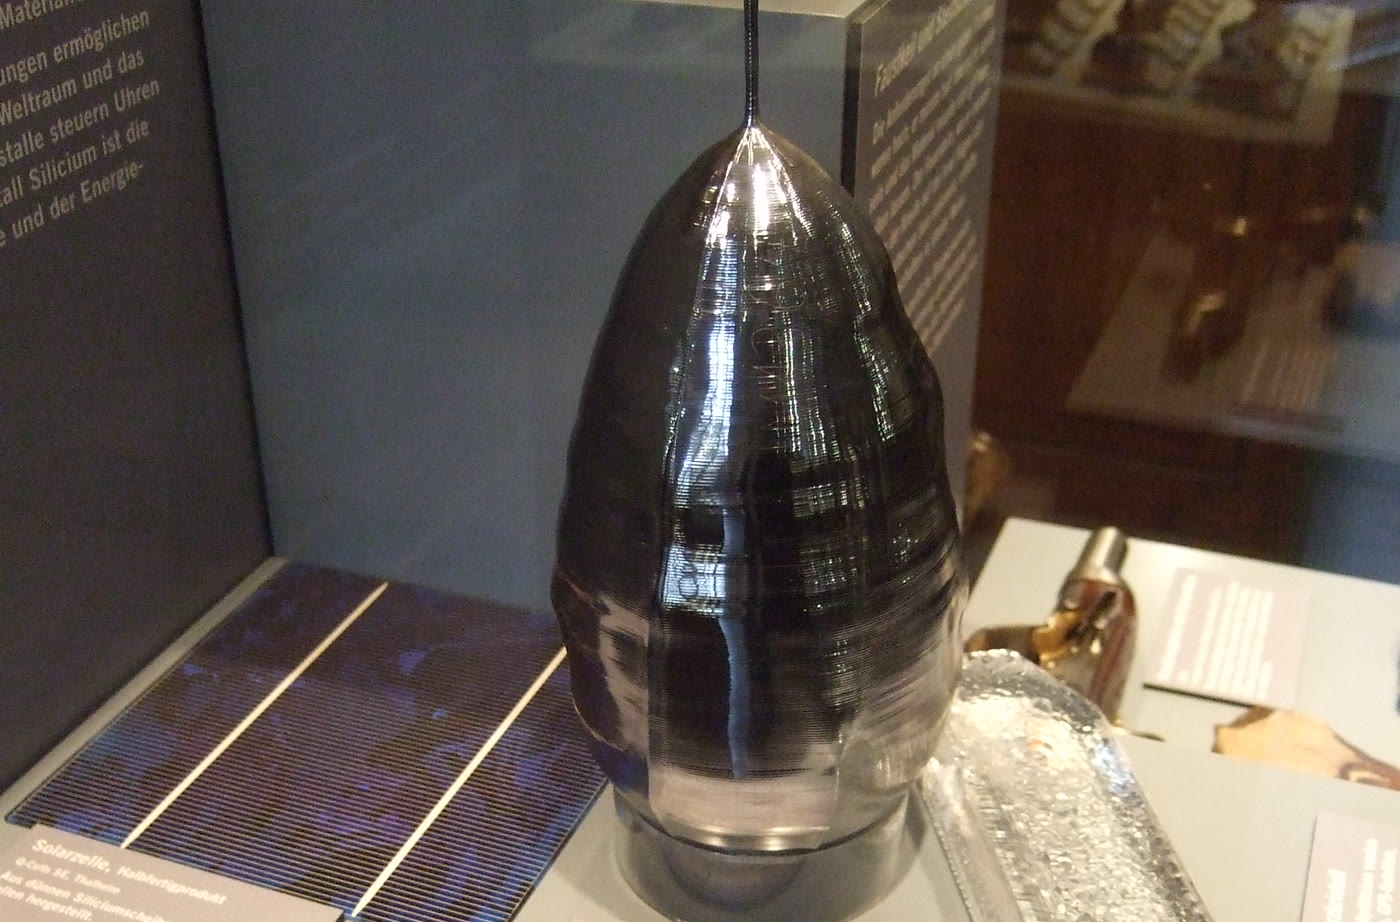
\includegraphics[width=0.5\linewidth]{images/book4/silicon-boule.jpg}

{\small Un monocristal de silicium tiré du bain fondu, présenté à côté d'une
cellule solaire faite d'une tranche d'un tel cristal. Photographie~:
Sebastian Wallroth, domaine public.}
\end{omfigure}

\begin{inthelab}[Faire croître un cristal de silicium]
Dans la méthode de Czochralski, du silicium polycristallin très pur est
fondu dans un creuset de silice sous argon, un peu au-dessus de son point
de fusion, le \omterm{def:b3:solid-state:doping}{dopant} étant ajouté au bain. Un petit germe cristallin fixé à
une tige en rotation est plongé dans le bain puis lentement remonté~: le
silicium cristallise sur lui avec l'orientation du germe, et les vitesses
de tirage et de rotation fixent le diamètre. Le lingot est ensuite scié en
plaquettes de moins d'un millimètre d'épaisseur. Le silane et les gaz
\omterm{def:b3:solid-state:doping}{dopants} phosphine et arsine utilisés aux étapes suivantes sont
pyrophoriques ou très toxiques, et ne sont manipulés que dans des
installations industrielles étanches.
\end{inthelab}

\section{Défauts ponctuels}

\begin{definition}[Défauts ponctuels]\label{def:b3:solid-state:defects}
Un \emph{défaut ponctuel}\index{defaut ponctuel@défaut ponctuel} est un écart au cristal parfait
localisé sur un site~: une lacune, un atome interstitiel ou un atome
étranger. Dans un cristal ionique, un \emph{défaut de Schottky}\index{defaut de Schottky@défaut de Schottky} est une
paire de lacunes, l'une cationique et l'autre anionique, les ions étant
partis vers la surface~; un \emph{défaut de Frenkel}\index{defaut de Frenkel@défaut de Frenkel} est une
paire formée d'une lacune et de l'ion qui l'a quittée, situé sur un site
interstitiel.
\end{definition}

\begin{omfigure}
\begin{tikzpicture}[scale=0.62]
  \begin{scope}
  \foreach \i in {0,...,5} \foreach \j in {0,...,4} {
    \pgfmathtruncatemacro{\pty}{mod(\i+\j,2)}
    \ifnum\pty=0 \fill[omDef!70] (\i,\j) circle (0.2); \else \fill[omThm!25] (\i,\j) circle (0.38); \draw[omThm!60] (\i,\j) circle (0.38); \fi
  }
  \fill[white] (2,2) circle (0.45); \draw[dashed] (2,2) circle (0.3);
  \fill[white] (3,2) circle (0.45); \draw[dashed] (3,2) circle (0.38);
  \node[font=\small\bfseries] at (2.5,5.0) {Schottky (NaCl)};
  \end{scope}
  \begin{scope}[xshift=8cm]
  \foreach \i in {0,...,5} \foreach \j in {0,...,4} {
    \pgfmathtruncatemacro{\pty}{mod(\i+\j,2)}
    \ifnum\pty=0 \fill[black!45] (\i,\j) circle (0.2); \else \fill[omMeth!25] (\i,\j) circle (0.38); \draw[omMeth!60] (\i,\j) circle (0.38); \fi
  }
  \fill[white] (2,2) circle (0.3); \draw[dashed] (2,2) circle (0.22);
  \fill[black!45] (2.5,2.5) circle (0.2);
  \draw[->, thick] (2.1,2.1) -- (2.38,2.38);
  \node[font=\small\bfseries] at (2.5,5.0) {Frenkel (AgCl)};
  \end{scope}
\end{tikzpicture}

{\small \omterm{def:b3:solid-state:defects}{Défauts ponctuels} dans une couche d'un cristal de type chlorure de
sodium (petits points~: cations~; grands cercles~: anions~; en tirets~:
lacunes). À gauche~: une paire de Schottky, un cation et un anion
manquants. À droite~: une paire de Frenkel, un ion argent déplacé de son
site vers une position interstitielle.}
\end{omfigure}

\begin{theorem}[Concentration d'équilibre des défauts de Schottky]\label{thm:b3:solid-state:schottky}
Dans un cristal MX de $N$ unités formulaires, le nombre $n$ de paires de
Schottky à l'équilibre, d'enthalpie de formation $\Delta H_S$ par paire et avec $n \ll N$, vaut
\[
  \frac{n}{N} = \eu^{-\Delta H_S/2kT}.
\]
\end{theorem}

\begin{proof}
La création de $n$ paires coûte $n\,\Delta H_S$ et apporte une entropie de configuration, due aux
$\binom{N}{n}$ façons de choisir les lacunes cationiques et à autant pour les anions~:
$S = 2k\ln\frac{N!}{n!(N - n)!}$. Avec la formule de Stirling $\ln x! \approx x\ln x - x$,
\[
  G(n) = n\,\Delta H_S - 2kT\bigl[N\ln N - n\ln n - (N - n)\ln(N - n)\bigr].
\]
À l'équilibre, $\dd G/\dd n = 0$~: $\Delta H_S - 2kT\ln\frac{N - n}{n} = 0$, donc $n/(N - n) = \eu^{-\Delta H_S/2kT}$, d'où $n/N$ pour
$n \ll N$. L'entropie vibrationnelle des défauts, négligée ici, multiplie le
résultat par un facteur constant.
\end{proof}

\begin{proposition}[Défauts de Frenkel]\label{prop:b3:solid-state:frenkel}
Avec $N$ ions de l'espèce mobile, $N_i$ sites interstitiels qui leur sont accessibles et
$\Delta H_F$ l'enthalpie de formation d'une paire, le nombre de paires de Frenkel vaut $n =
\sqrt{NN_i}\,\eu^{-\Delta H_F/2kT}$ (pour $n \ll N, N_i$).
\end{proposition}

\begin{proof}
L'entropie s'écrit maintenant $S = k\ln\binom{N}{n} + k\ln\binom{N_i}{n}$, et la même minimisation donne
\[
  \Delta H_F = kT\ln\frac{(N - n)(N_i - n)}{n^2} \approx kT\ln\frac{NN_i}{n^2},
\]
d'où le résultat.
\end{proof}

La racine carrée montre que les défauts se forment par paires~: comme $n_i$
dans un \omterm{def:b3:solid-state:classes}{semi-conducteur}, leur concentration a la moitié de l'énergie de
formation dans son exposant. Les halogénures alcalins forment surtout des
\omterm{def:b3:solid-state:defects}{défauts de Schottky}~; les halogénures d'argent, dont le petit ion
$\ce{Ag+}$, polarisable, se glisse entre les anions, surtout des \omterm{def:b3:solid-state:defects}{défauts de Frenkel}.

\begin{definition}[Notation de Kröger--Vink]\label{def:b3:solid-state:kroger-vink}
La \emph{notation de Kröger--Vink}\index{notation de Kroger--Vink@notation de Kröger--Vink} écrit un \omterm{def:b3:solid-state:defects}{défaut ponctuel}
sous la forme $\mathrm{A_S^c}$~: A est l'espèce présente sur le site (V pour une lacune, $i$ comme site
pour un interstitiel), S le site qu'elle occupe dans le cristal parfait, et c sa
charge relative à ce site~: $\bullet$ pour chaque unité positive, $'$ pour chaque unité
négative, $\times$ pour une charge nulle.
\end{definition}

Ainsi, $\mathrm{V_{Na}'}$ est une lacune de sodium (le $+1$ manquant laisse une charge relative $-1$),
$\mathrm{V_{Cl}^{\bullet}}$ une lacune de chlorure, $\mathrm{Ag_i^{\bullet}}$ un ion argent interstitiel, $\mathrm{Ca_{Na}^{\bullet}}$ un ion calcium sur un
site de sodium, $\mathrm{O_O^{\times}}$ un ion oxyde à sa place. L'équilibre de Schottky de NaCl s'écrit
$\text{rien} \rightleftharpoons \mathrm{V_{Na}' + V_{Cl}^{\bullet}}$, l'équilibre de Frenkel de AgCl
$\mathrm{Ag_{Ag}^{\times}} \rightleftharpoons \mathrm{Ag_i^{\bullet} + V_{Ag}'}$.

\begin{method}[Écrire une équation de défauts]\label{met:b3:solid-state:kroger-vink}
\begin{enumerate}
  \item Écrire ce qui est ajouté au cristal hôte et les défauts que cela
        crée.
  \item Bilan des sites~: le rapport des sites cationiques aux sites
        anioniques de l'hôte est conservé (les lacunes comptent comme des
        sites).
  \item Bilan de matière~: les mêmes atomes des deux côtés (les lacunes
        n'ont pas de masse~; les électrons $e'$ et les \omterm{def:b3:solid-state:carriers}{trous} $h^\bullet$ non plus).
  \item Bilan des charges~: les sommes des charges effectives sont égales.
\end{enumerate}
\end{method}

\begin{example}[L'oxyde d'yttrium dans la zircone]
Dissoudre $\ce{Y2O3}$ dans $\ce{ZrO2}$ place deux $\ce{Y^3+}$ sur des sites $\ce{Zr^4+}$, chacun de charge relative $-1$, et
trois ions oxyde sur des sites d'oxygène~; le rapport de l'hôte, un site
cationique pour deux sites d'oxygène, exige quatre sites d'oxygène pour les
deux cations, si bien que l'un d'eux reste vide~:
\[
  \ce{Y2O3} \xrightarrow{\ce{ZrO2}} \mathrm{2\,Y_{Zr}' + 3\,O_O^{\times} + V_O^{\bullet\bullet}}.
\]
Sites~: 2 cationiques, 4 d'oxygène~; matière~: 2 Y et 3 O~; charge~: $2(-1) + 2 = 0$. Une lacune
d'oxyde pour deux ions yttrium~: c'est ce qui fait de la zircone stabilisée
à l'oxyde d'yttrium un conducteur par ions oxyde.
\end{example}

\begin{definition}[Centre coloré]\label{def:b3:solid-state:colour-centre}
Un \emph{centre coloré}\index{centre colore@centre coloré} est un \omterm{def:b3:solid-state:defects}{défaut ponctuel} qui absorbe
la lumière visible, comme un électron piégé dans une lacune anionique d'un
halogénure alcalin (un centre F), qui colore un cristal par ailleurs
transparent.
\end{definition}

Chauffer du chlorure de sodium dans de la vapeur de sodium ou l'irradier
crée des centres F~: l'électron piégé se comporte comme une \omterm{def:b3:quantum-model-systems:box}{particule dans
une boîte} de la taille de la lacune et absorbe dans le visible, ce qui
colore le cristal en brun jaune.

\section{Non-stœchiométrie}

\begin{definition}[Composés non stœchiométriques]\label{def:b3:solid-state:non-stoichiometric}
Un \emph{composé non stœchiométrique}\index{compose non stoechiometrique@composé non stœchiométrique} est un
solide dont la composition varie dans un domaine autour d'un rapport simple
de nombres entiers, l'écart étant absorbé par des \omterm{def:b3:solid-state:defects}{défauts ponctuels}.
\end{definition}

L'oxyde de fer(II) n'est jamais exactement $\ce{FeO}$~: il est toujours déficitaire en fer,
$\mathrm{Fe_{1-x}O}$, avec un $x$ fixé par la température et la pression d'oxygène auxquelles il a été préparé. Chaque $\ce{Fe^2+}$ manquant est compensé par deux
$\ce{Fe^3+}$, qui sont, dans le langage des défauts, des \omterm{def:b3:solid-state:carriers}{trous} sur des sites de fer.

\begin{proposition}[Conductivité et pression d'oxygène]\label{prop:b3:solid-state:brouwer}
Pour un oxyde déficitaire en métal $\mathrm{M_{1-x}O}$ dont les défauts sont des lacunes métalliques doublement
chargées compensées par des \omterm{def:b3:solid-state:carriers}{trous}, la concentration en \omterm{def:b3:solid-state:carriers}{trous}, et la
conductivité, varient comme
$p(\ce{O2})^{1/6}$. Pour un oxyde déficitaire en oxygène compensé par des électrons, elles varient comme
$p(\ce{O2})^{-1/6}$.
\end{proposition}

\begin{proof}
L'absorption d'oxygène crée des lacunes métalliques~:
\[
  \tfrac12\ce{O2} \rightleftharpoons \mathrm{O_O^{\times} + V_M'' + 2\,h^{\bullet}}, \qquad K = \frac{[\mathrm{V_M''}][\mathrm h^\bullet]^2}{p(\ce{O2})^{1/2}}
\]
(l'activité de $\mathrm{O_O^{\times}}$ vaut 1). Le
bilan des charges s'écrit $[\mathrm h^\bullet] = 2[\mathrm{V_M''}]$, donc $[\mathrm h^\bullet]^3 = 2K\,p(\ce{O2})^{1/2}$ et $[\mathrm h^\bullet] \propto p(\ce{O2})^{1/6}$. Dans le
cas déficitaire en oxygène, $\mathrm{O_O^{\times}} \rightleftharpoons \tfrac12\ce{O2} + \mathrm{V_O^{\bullet\bullet} + 2\,e'}$, $[\mathrm e'] = 2[\mathrm{V_O^{\bullet\bullet}}]$, et les mêmes étapes donnent $[\mathrm e'] \propto p(\ce{O2})^{-1/6}$.
La conductivité est proportionnelle à la concentration en porteurs.
\end{proof}

Le tracé de $\log\sigma$ en fonction de $\log p(\ce{O2})$ indique ainsi quels défauts dominent~: sa pente,
$\pm 1/4$ ou $\pm 1/6$, dépend de leurs charges.

\section{Conducteurs ioniques}

\begin{definition}[Conducteurs ioniques]\label{def:b3:solid-state:ionic-conductor}
Un \emph{conducteur ionique}\index{conducteur ionique} est un solide dans
lequel le courant est porté par des ions qui se déplacent à travers le
réseau. Un \emph{électrolyte solide}\index{electrolyte solide@électrolyte solide} est un conducteur ionique
dont la conductivité électronique est négligeable, si bien qu'il peut
séparer les deux électrodes d'une cellule électrochimique.
\end{definition}

\begin{proposition}[Loi d'Arrhenius de la conduction ionique]\label{prop:b3:solid-state:ionic-arrhenius}
Pour des ions qui se déplacent par sauts entre sites voisins au-dessus d'une barrière $E_a$,
$\sigma T = A\,\eu^{-E_a/kT}$.
\end{proposition}

\begin{proof}[Démonstration partielle]
Un ion tente des sauts à une fréquence $\nu_0$ et réussit avec une probabilité $\eu^{-E_a/kT}$,
si bien que son coefficient de diffusion vaut $D = \tfrac16\nu_0 z a^2\eu^{-E_a/kT}$ pour $z$ sites voisins à
la distance $a$ (marche aléatoire). La relation de Nernst--Einstein $\sigma = nq^2D/kT$ (admise), pour $n$
ions mobiles de charge $q$ par unité de volume, donne $\sigma T = (nq^2\nu_0za^2/6k)\,\eu^{-E_a/kT}$. La
concentration $n$ est fixée par le dopage dans un conducteur extrinsèque~;
lorsqu'elle est elle-même créée thermiquement, $E_a$ contient aussi la moitié de l'enthalpie de formation.
\end{proof}

% ledger: trans:AgI
Trois \omterm{def:b3:solid-state:ionic-conductor}{électrolytes solides} illustrent l'éventail. Dans la zircone
stabilisée à l'oxyde d'yttrium, les lacunes d'oxyde créées par le \omterm{def:b3:solid-state:doping}{dopant}
permettent aux ions $\ce{O^2-}$ de sauter~; elle ne conduit utilement qu'à chaud, à
plusieurs centaines de degrés Celsius. Dans l'alumine $\beta$, les ions sodium se déplacent dans
des plans peu denses entre des blocs spinelle, à la base des batteries
sodium--soufre. L'iodure d'argent devient un conducteur superionique
au-dessus de \qty{146}{\celsius}, température où ses ions argent se
répartissent sur bien plus de sites qu'il n'y a d'ions, presque comme un
liquide dans un réseau rigide d'iodure. Les conducteurs d'ions lithium
(grenats de zirconate de lithium et de lanthane, sulfures) sont les
électrolytes des batteries tout solide aujourd'hui en développement.

\begin{omfigure}
\begin{tikzpicture}[font=\small, >=Stealth]
  \fill[omProp!25] (0,0) rectangle (2.4,3.2);
  \node[font=\scriptsize, align=center] at (1.2,0.6) {$\ce{ZrO2}$--$\ce{Y2O3}$\\ électrolyte solide};
  \draw[black!60, line width=2.5pt] (-0.07,0) -- (-0.07,3.2);
  \draw[black!60, line width=2.5pt] (2.47,0) -- (2.47,3.2);
  \node[font=\scriptsize, align=center] at (-2.0,1.4) {gaz d'échappement\\ $p(\ce{O2})$ faible};
  \node[font=\scriptsize, align=center] at (4.4,1.4) {air de référence\\ $p(\ce{O2}) = \qty{0.21}{bar}$};
  \node[font=\scriptsize, anchor=north] at (-0.07,-0.05) {Pt};
  \node[font=\scriptsize, anchor=north] at (2.47,-0.05) {Pt};
  \draw[->, thick, omThm] (2.0,1.9) -- (0.4,1.9) node[midway, above, font=\scriptsize] {$\ce{O^2-}$};
  \node[font=\scriptsize, anchor=west] at (2.65,2.75) {$\ce{O2 + 4e- -> 2O^2-}$};
  \node[font=\scriptsize, anchor=east] at (-0.25,2.75) {$\ce{2O^2- -> O2 + 4e-}$};
  \draw (-0.07,3.2) -- (-0.07,4.0) -- (0.85,4.0);
  \draw (2.47,3.2) -- (2.47,4.0) -- (1.55,4.0);
  \draw (1.2,4.0) circle (0.35) node {V};
\end{tikzpicture}

{\small La sonde à oxygène en zircone, en coupe~: des électrodes poreuses de
platine sur les deux faces de l'\omterm{def:b3:solid-state:ionic-conductor}{électrolyte solide}, l'une dans les gaz
d'échappement et l'autre dans l'air. Les ions oxyde transportent le courant
à travers l'électrolyte~; la tension mesure le rapport des deux pressions
d'oxygène.}
\end{omfigure}

\begin{history}[Le transistor et le cristal tiré]
En 1947, John Bardeen et Walter Brattain, dans le groupe de William
Shockley aux Bell Laboratories, réalisèrent le premier transistor à partir
d'un cristal de germanium~; tous trois partagèrent le prix Nobel de
physique 1956. Les cristaux provenaient d'une méthode que Jan Czochralski
avait trouvée en 1916 en mesurant la vitesse de cristallisation des métaux,
en tirant un fil d'étain du bain fondu~: adaptée au germanium puis au
silicium, elle produit encore les plaquettes de presque tous les circuits
intégrés.
\end{history}

\section{Exercices}

\begin{exercise}[$\star$]\label{exo:b3:solid-state:1}
Donner les six niveaux de Hückel d'une chaîne de six atomes en unités de $|\beta|$, et la
largeur du domaine qu'ils couvrent.
\end{exercise}

\begin{exercise}[$\star$]\label{exo:b3:solid-state:2}
Combien d'électrons contient une bande construite à partir des orbitales s
de $N$ atomes~? Pourquoi le sodium et le magnésium sont-ils tous deux
métalliques~?
\end{exercise}

\begin{exercise}[$\star$]\label{exo:b3:solid-state:3}
Estimer la longueur d'onde de la lumière émise par des diodes au phosphure
de gallium (\qty{2.26}{eV}) et au nitrure de gallium (\qty{3.4}{eV}), à l'aide de $\lambda \approx hc/E_g$.
\end{exercise}

\begin{exercise}[$\star$]\label{exo:b3:solid-state:4}
Écrire les équations de Kröger--Vink de la dissolution de $\ce{CaCl2}$ dans $\ce{NaCl}$ et de $\ce{Y2O3}$ dans $\ce{ZrO2}$, et
vérifier chaque bilan.
\end{exercise}

\begin{exercise}[$\star\star$]\label{exo:b3:solid-state:5}
Avec $N_c = \num{6.2e15}\,T^{3/2}$, $N_v = \num{3.5e15}\,T^{3/2}$ (en $\unit{cm^{-3}}$) et $E_g = \qty{1.125}{eV}$ pour le silicium à \qty{300}{K},
et $N_c = \num{1.98e15}\,T^{3/2}$, $N_v = \num{9.6e14}\,T^{3/2}$, $E_g = \qty{0.661}{eV}$ pour le germanium, calculer $n_i$ pour chacun, ainsi que leur
rapport.
\end{exercise}

\begin{exercise}[$\star\star$]\label{exo:b3:solid-state:6}
Le silicium est dopé par $\qty{1.0e16}{cm^{-3}}$ de phosphore. Avec $n_i = \qty{1.0e10}{cm^{-3}}$ à \qty{300}{K}, donner les
concentrations en électrons et en \omterm{def:b3:solid-state:carriers}{trous}.
\end{exercise}

\begin{exercise}[$\star\star$]\label{exo:b3:solid-state:7}
Pour le cristal de l'\cref{exo:b3:solid-state:6}, de combien le \omterm{def:b3:solid-state:fermi}{niveau de
Fermi} se situe-t-il au-dessus du niveau intrinsèque~?
\end{exercise}

\begin{exercise}[$\star\star$]\label{exo:b3:solid-state:8}
L'enthalpie de formation d'une paire de Schottky dans NaCl vaut environ
\qty{2.3}{eV} (données de l'exercice). Calculer la fraction de sites
vacants à \qty{800}{K}, et le nombre de paires dans une mole.
\end{exercise}

\begin{exercise}[$\star\star$]\label{exo:b3:solid-state:9}
Un échantillon d'oxyde de fer(II) (structure de type chlorure de sodium,
quatre sites d'oxygène par maille) a
$a = \qty{430.0}{pm}$ et une masse volumique de \qty{5.70}{g.cm^{-3}} (données de l'exercice). En supposant
les sites d'oxygène tous occupés, trouver $x$ dans $\mathrm{Fe_{1-x}O}$.
\end{exercise}

\begin{exercise}[$\star\star\star$]\label{exo:b3:solid-state:10}
Un conducteur d'ions lithium a $\sigma = \qty{1.0e-4}{S.cm^{-1}}$ à \qty{300}{K}, $\qty{7.8e-4}{S.cm^{-1}}$ à \qty{350}{K} et
$\qty{3.6e-3}{S.cm^{-1}}$ à \qty{400}{K} (données de l'exercice). Trouver son énergie d'activation.
\end{exercise}

\begin{exercise}[$\star\star\star$]\label{exo:b3:solid-state:11}
Montrer que, dans un oxyde dont les défauts dominants sont des lacunes
métalliques simplement chargées
$\mathrm{V_M'}$ compensées par des \omterm{def:b3:solid-state:carriers}{trous}, la conductivité varie comme $p(\ce{O2})^{1/4}$.
\end{exercise}

\begin{exercise}[$\star\star\star$]\label{exo:b3:solid-state:12}
Dans AgCl, la paire de Frenkel a une enthalpie de formation d'environ
\qty{1.4}{eV}, et il y a deux sites interstitiels par ion argent (données
de l'exercice). Calculer la fraction des ions argent situés sur des sites
interstitiels à \qty{600}{K}.
\end{exercise}

\section{Problème~: la sonde à oxygène d'un pot d'échappement}

\begin{problem}[{Problème du week-end --- la sonde à oxygène d'un pot
d'échappement~: les défauts de la zircone stabilisée à l'oxyde d'yttrium,
sa conductivité ionique et sa température de fonctionnement, la tension de
Nernst de la cellule, et la bascule entre gaz d'échappement pauvres et
riches}]
\label{pb:b3:solid-state:1}
% ledger: const:R, const:F, const:kB, const:e, const:NA, air:O2
L'électrolyte de la sonde est de la zircone à 8.0\,mol\,\% de $\ce{Y2O3}$, de structure fluorine
avec quatre sites cationiques et huit sites d'oxygène par maille cubique, $a = \qty{514}{pm}$~; un disque
de \qty{1.0}{mm} d'épaisseur et de \qty{0.20}{cm^2} de surface sépare les
gaz d'échappement de l'air. Sa
conductivité suit $\sigma T = A\eu^{-E_a/kT}$ avec $E_a = \qty{1.0}{eV}$ et $\sigma = \qty{0.030}{S.cm^{-1}}$ à \qty{800}{\celsius}. Les gaz
d'échappement pauvres ont $p(\ce{O2}) = \qty{0.010}{bar}$, les gaz riches $p(\ce{O2}) = \qty{1.0e-20}{bar}$ (toutes données du problème).

\medskip\noindent\textbf{Partie I --- L'électrolyte.}
\begin{enumerate}
  \item Écrire l'équation de Kröger--Vink de la dissolution de $\ce{Y2O3}$ dans $\ce{ZrO2}$.
  \item Vérifier ses bilans de sites, de matière et de charges.
  \item Combien de lacunes d'oxyde sont créées par ion yttrium~?
  \item Écrire la composition sous la forme $\mathrm{Zr_{1-x}Y_xO_{2-x/2}}$ et calculer $x$.
  \item Calculer la fraction des sites d'oxygène qui sont vacants.
  \item Calculer le nombre de lacunes par maille.
  \item Calculer la concentration en lacunes en $\unit{cm^{-3}}$.
\end{enumerate}

\medskip\noindent\textbf{Partie II --- Conductivité et température.}
\begin{enumerate}[resume]
  \item Pourquoi la conductivité croît-elle fortement avec la température~?
  \item Calculer $A$.
  \item Calculer $\sigma$ à \qty{700}{\celsius}.
  \item Calculer $\sigma$ à \qty{300}{\celsius}.
  \item Calculer la résistance du disque à ces deux températures.
  \item L'électronique exige une résistance inférieure à \qty{1}{k\ohm}~:
        trouver la température de fonctionnement la plus basse.
  \item Pourquoi ces sondes sont-elles munies d'un élément chauffant~?
\end{enumerate}

\medskip\noindent\textbf{Partie III --- La tension de Nernst.}
\begin{enumerate}[resume]
  \item Écrire la réaction d'électrode du côté de l'air, en notation
        ordinaire et en \omterm{def:b3:solid-state:kroger-vink}{notation de Kröger--Vink}.
  \item Montrer que la tension de la cellule vaut $E = (RT/4F)\ln\bigl(p_{\mathrm{air}}/p_{\mathrm{exh}}\bigr)$.
  \item Calculer $RT/4F$ à \qty{700}{\celsius}.
  \item Quelle est la tension si les gaz d'échappement contenaient de
        l'air~?
  \item Calculer la variation de tension pour un facteur dix sur $p(\ce{O2})$.
\end{enumerate}

\medskip\noindent\textbf{Partie IV --- Pauvre, riche et la bascule.}
\begin{enumerate}[resume]
  \item Calculer la tension dans des gaz d'échappement pauvres à
        \qty{700}{\celsius}.
  \item Calculer la tension dans des gaz d'échappement riches à
        \qty{700}{\celsius}.
  \item Pourquoi $p(\ce{O2})$ est-elle si faible dans les gaz d'échappement riches~?
  \item Le calculateur du moteur bascule à \qty{0.45}{V}~: à quelle
        pression d'oxygène cela correspond-il~?
  \item Pourquoi la tension saute-t-elle au rapport air/carburant
        stœchiométrique, et comment le calculateur du moteur
        l'utilise-t-il~?
  \item Énoncer le résultat~: la tension de la sonde dans des gaz
        d'échappement riches à \qty{700}{\celsius}.
\end{enumerate}
\end{problem}
